\section{Results}

\begin{table}[H]
\centering
\caption{Run times for MC method and RK4 method with 10$^5$ integration points and 30 stochastic simulations}
\begin{tabular}{|l|l|l|l|}
\hline
Simulation Time & Average MC [s] & All MC [s]& RK4 [s]\\
\hline
10 & 0.0998 & 2.996 & 1.721 \\
100 & 0.978 & 29.351 & 1.779\\
1000 & 10.182 & 305.479 & 1.723\\
\hline
\end{tabular}
\label{tab:Run_times}
\end{table}

Computational execution times for the program is presented in Table \ref{tab:Run_times}. "Average MC" shows the average time for each Monte Carlo simulation across 30 simulations, while "All MC" pertains to the total time for all 100 simulations. As can plainly be seen from the table, while the computational time for the average Monte Carlo simulation increases linearly, the Runge-Kutta solver is more or less constant for admittedly pretty short simulations. Simulations with times beyond 1000 are unnecessary to show here, as the differences between Monte Carlo and Runge-Kutta are obvious. 

%Plots for kjøring uten vital, og fractions
 \begin{figure}[H]
		\centering
		\begin{subfigure}{0.49\linewidth}
			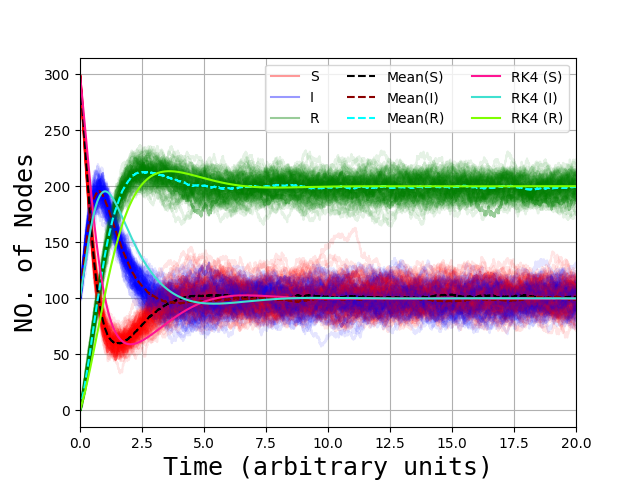
\includegraphics[width=1.1\linewidth]{Figures/OppgA_4_1_05.png}
			\caption{$\beta = 1$}
		\end{subfigure}
		\begin{subfigure}{0.49\linewidth}
			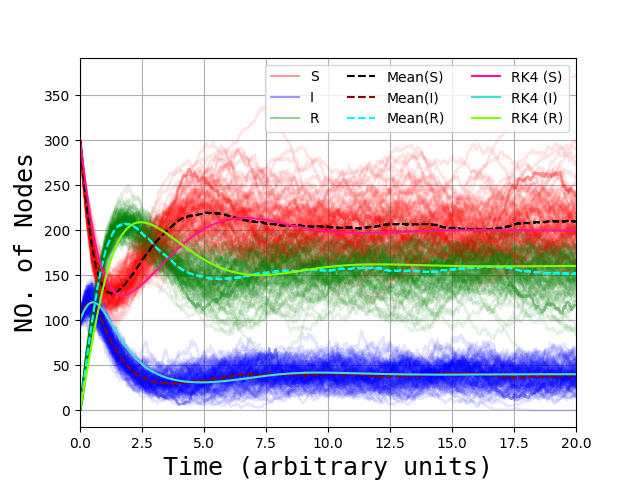
\includegraphics[width=1.1\linewidth]{Figures/OppgA_4_2_05.png}
			\caption{$\beta = 2$}
		\end{subfigure}
		\begin{subfigure}{0.49\linewidth}
			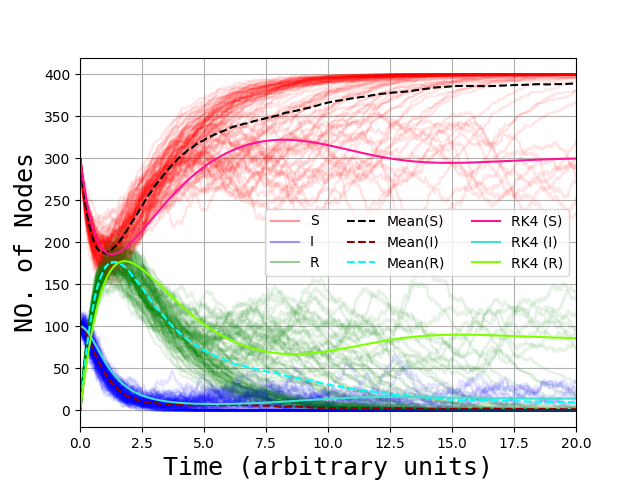
\includegraphics[width=1.1\linewidth]{Figures/OppgA_4_3_05.png}
			\caption{$\beta = 3$}
		\end{subfigure}
		\begin{subfigure}{0.49\linewidth}
		    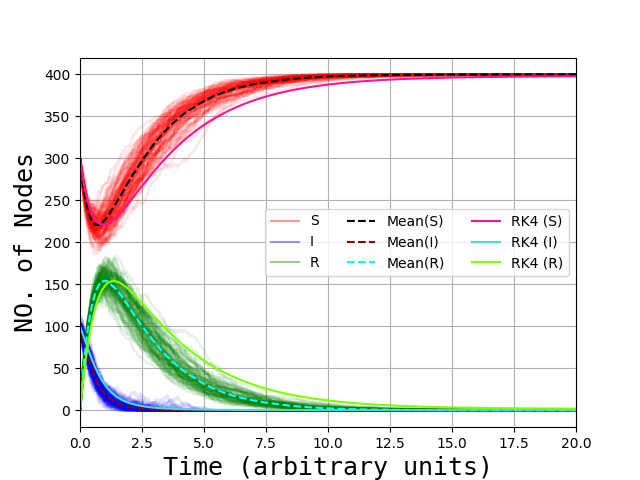
\includegraphics[width=1.1\linewidth]{Figures/OppgA_4_4_05.png}
			\caption{$\beta = 4$}
		\end{subfigure}
		\caption{Temporal development of the S, I and R populations, with different initial value for $\beta$, the rate of recovery. $\alpha = 4$ and $\gamma = 0.5$}
		\label{fig:1}
	\end{figure}
	
The four plots in Figure \ref{fig:1} shows the development of the populations of S, I and R with time with different values of $\beta$ for each plot. The values for $\alpha$ and $\gamma$ are held constant. For each plot, the Monte Carlo simulation has been run 100 times. These are the fine red, green and blue lines with varying degree of hue seen in the plots. This allows a deeper shade of color to be interpreted as statistically more common outcomes. The dashed lines show the expectation values at each point in time between all the simulations. The solid lines correspond to the Runge-Kutta solutions.

\begin{table}[H]
\centering	
\begin{tabular}{|c||c|c|c|c|}
\hline
\multicolumn{5}{|c|}{S}\\
\hline
$\beta$&1&2&3&4\\
\hline\hline
$S_\infty$& 100 & 200 & 300 & 400\\
\hline
RK4& 99.75 & 199.90 & 300.24& 397.80\\
\hline
MC& 101.94 & 207.51 & 380.68 & 399.98\\
\hline
\end{tabular}
\begin{tabular}{|c||c|c|c|c|}
\hline
\multicolumn{5}{|c|}{I}\\
\hline
$\beta$&1&2&3&4\\
\hline\hline
$I_\infty$& 100 & 40 & 14.28 & 0 \\
\hline
RK4& 100.08 & 40.07 & 14.06 & 0.21\\
\hline
MC& 98.21 & 37.22 & 1.98 & 0.0\\
\hline
\end{tabular}
\begin{tabular}{|c||c|c|c|c|}
\hline
\multicolumn{5}{|c|}{R}\\
\hline
$\beta$&1&2&3&4\\
\hline\hline
$R_\infty$& 200 & 160 & 85.71 & 0\\
\hline
RK4& 200.17 & 160.03 & 85.70 & 1.99\\
\hline
MC& 199.85 & 155.27 & 17.34 & 0.02\\
\hline
\end{tabular}
\caption{Expectation values for Monte Carlo simulations after equilibration. The final corresponding Runge-Kutta value, and the fraction of people in each population at equilibrium, for each value of $\beta$.}
\label{table:2}
\end{table}

Table \ref{table:2} shows the total number of agents occupying each compartment at equilibrium for each of the four different networks as computed by the expressions in \eqref{sirseq}. This is compared to the final value from the plots in Figure \ref{fig:1}, where "RK4" is the value obtained from the Runge-Kutta solver, and "MC" is the expectation value acquired across all 100 simulations. 



\begin{table}[H]
\centering
\begin{tabular}{|c||l|l||l|l||l|l|}
\hline
\multirow{2}{*}{$\beta$}
    & \multicolumn{2}{c||}{S}
        & \multicolumn{2}{|c||}{I}
            & \multicolumn{2}{|c|}{R} \\   \cline{2-7}
 & $\sigma$ & $\bar{x}$ & $\sigma$ & $\bar{x}$ & $\sigma$ & $\bar{x}$\\ \hline
 1&11.62&101.94&12.39&98.21&9.30&199.85 \\ \hline
 2&29.70&207.51&13.02&37.22&1.99&155.27 \\ \hline
 3&23.96&380.68&3.22&1.98&21.29&17.34 \\ \hline
 4&0.14&399.98&0.0&0.0&0.14&0.02 \\ \hline
\end{tabular}
\caption{Expectation values $\bar{x}$ and standard deviations $\sigma$ for the Monte Carlo simulations after equilibrium.}
\label{table:3}
\end{table}
Table \ref{table:3} shows the expectation values across 100 Monte Carlo simulations at equilibrium as well as the standard deviation, for varying values of $\beta$. 

%VITAL DYNAMICS
 \begin{figure}[H]
		\centering
		\begin{subfigure}{0.49\linewidth}
			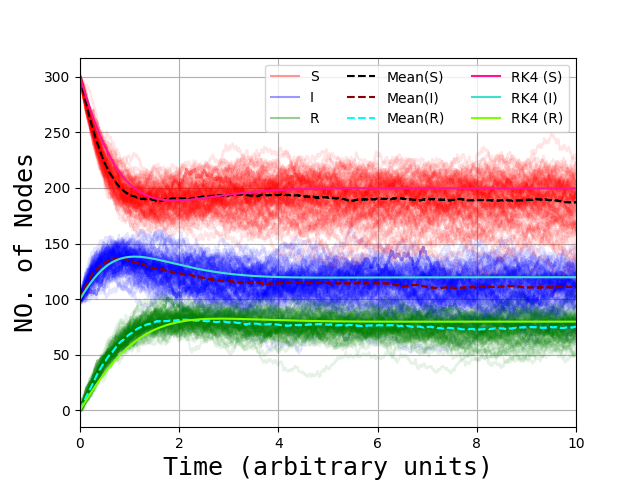
\includegraphics[width=1.1\linewidth]{Figures/OppgB_1_0_1.png}
			\caption{$\alpha = 4$, $\beta = 1$, $\gamma=0.5$, $\mu=1$, $\mu^*=0$, $\epsilon=1$}
		\end{subfigure}
		\begin{subfigure}{0.49\linewidth}
			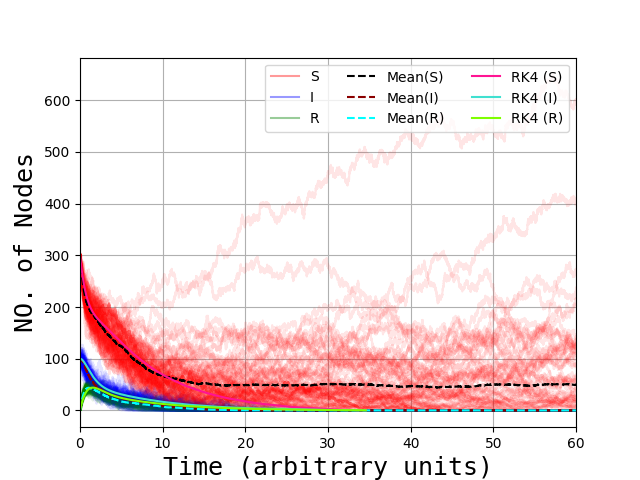
\includegraphics[width=1.1\linewidth]{Figures/OppgB_1_1_1.png}
			\caption{$\alpha = 4$, $\beta = 1$, $\gamma=0.5$, $\mu=1$, $\mu^*=1$, $\epsilon=1$}
		\end{subfigure}
		\begin{subfigure}{0.49\linewidth}
			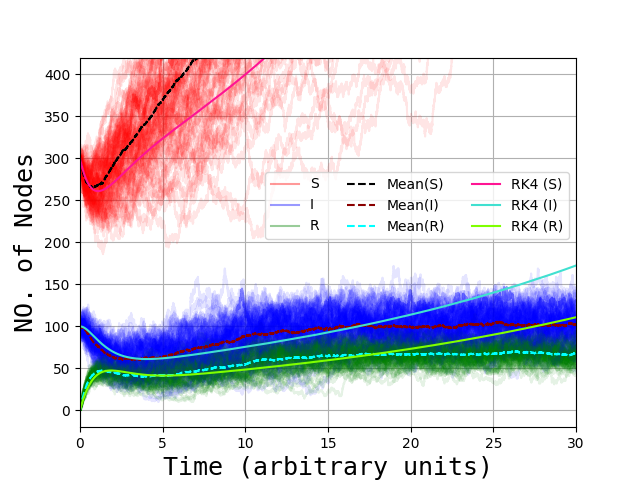
\includegraphics[width=1.1\linewidth]{Figures/OppgB_1_1_12.png}
			\caption{$\alpha = 4$, $\beta = 1$, $\gamma=0.5$, $\mu=1$, $\mu^*=1$, $\epsilon=1.2$}
		\end{subfigure}
		\begin{subfigure}{0.49\linewidth}
		    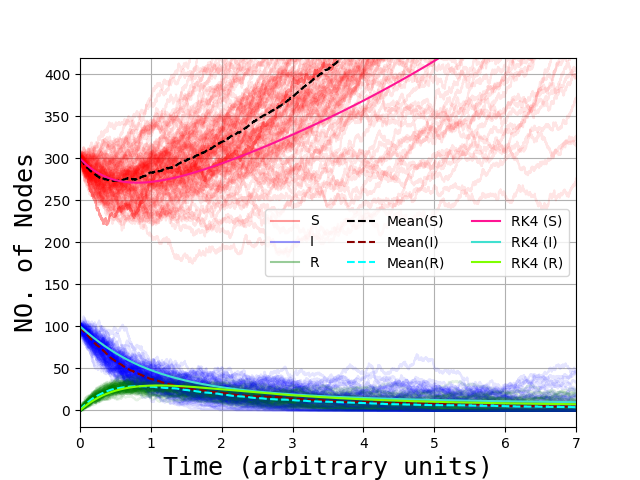
\includegraphics[width=1.1\linewidth]{Figures/OppgB_1_2_12.png}
			\caption{$\alpha = 4$, $\beta = 1$, $\gamma=0.5$, $\mu=1$, $\mu^*=2$, $\epsilon=1.2$}
		\end{subfigure}
		\caption{Temporal development of the S, I and R populations, with vital dynamics modelled.}
		\label{fig:vitaldynamics}
	\end{figure}
	
Figure \ref{fig:vitaldynamics} have the SIR-models with vital dynamics enabled. The variables $\mu$, $\mu^*$ and $\epsilon$ govern the conditions respectively for death from natural causes, death from infection, and the birth rate.

%SEASONAL VARIATION
 \begin{figure}[H]
		\centering
		\begin{subfigure}{0.49\linewidth}
			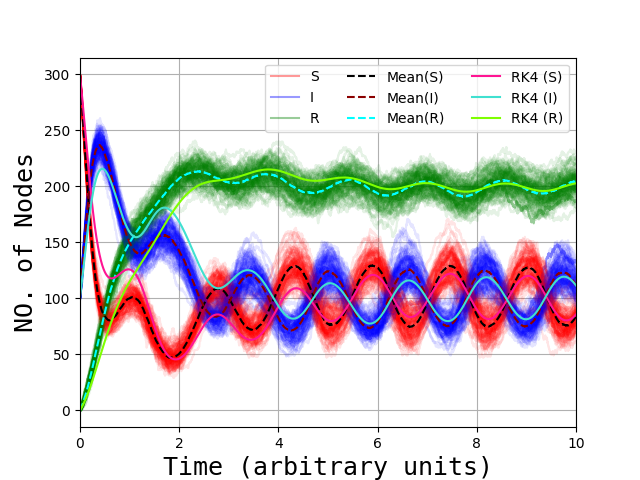
\includegraphics[width=1.1\linewidth]{Figures/OppgC_4_4.png}
			\caption{$\alpha_0 = 4$, $A = 4$, $\omega = 4$}
		\end{subfigure}
		\begin{subfigure}{0.49\linewidth}
			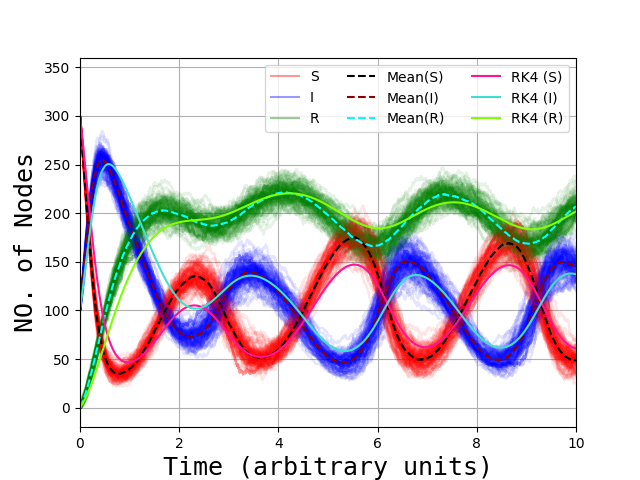
\includegraphics[width=1.1\linewidth]{Figures/OppgC_4_2.png}
			\caption{$\alpha_0 = 4$, $A = 4$, $\omega = 2$}
		\end{subfigure}
		\begin{subfigure}{0.49\linewidth}
			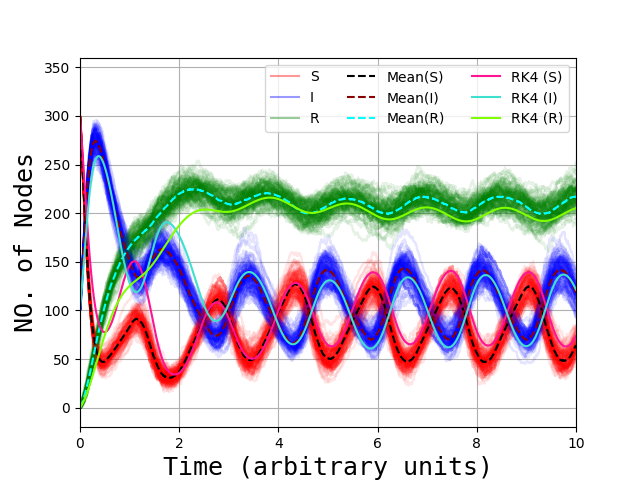
\includegraphics[width=1.1\linewidth]{Figures/OppgC_8_4.png}
			\caption{$\alpha_0 = 4$, $A = 8$, $\omega = 4$}
		\end{subfigure}
		\begin{subfigure}{0.49\linewidth}
		    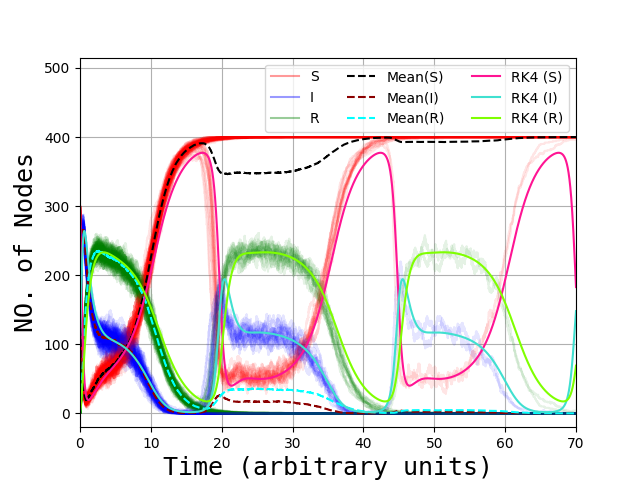
\includegraphics[width=1.1\linewidth]{Figures/OppgC_4_025.png}
			\caption{$\alpha_0 = 4$, $A = 4$, $\omega = 0.25$}
		\end{subfigure}
		\caption{Development with seasonal variation enabled. Different values for $A$ and $\omega$ have been used.}
		\label{fig:seasonalvar}
	\end{figure}
Figure \ref{fig:seasonalvar} displays four different simulations of the spread of disease in a network where we enable seasonal variation in the rate of infection, $\alpha(t)$. 
%Vaccination
 \begin{figure}[H]
		\centering
		\begin{subfigure}{0.49\linewidth}
			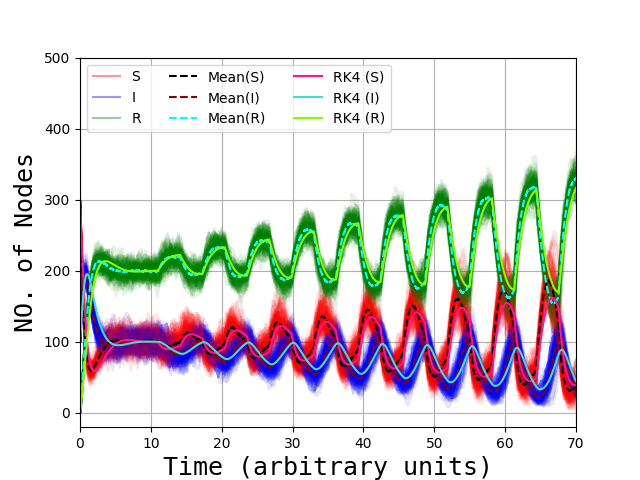
\includegraphics[width=1.1\linewidth]{Figures/Vax_Pulse2t_ckonst_4_1_05.png}
			\caption{Pulse vaccination, constant $\gamma$}
		\end{subfigure}
		\begin{subfigure}{0.49\linewidth}
			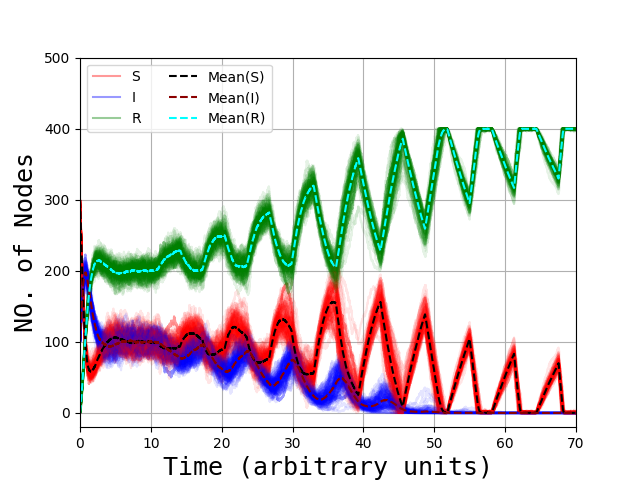
\includegraphics[width=1.1\linewidth]{Figures/Vax_Pulse2t_cvar_4_1_05.png}
			\caption{Pulse vaccination, variable $\gamma$}
		\end{subfigure}
		\begin{subfigure}{0.49\linewidth}
			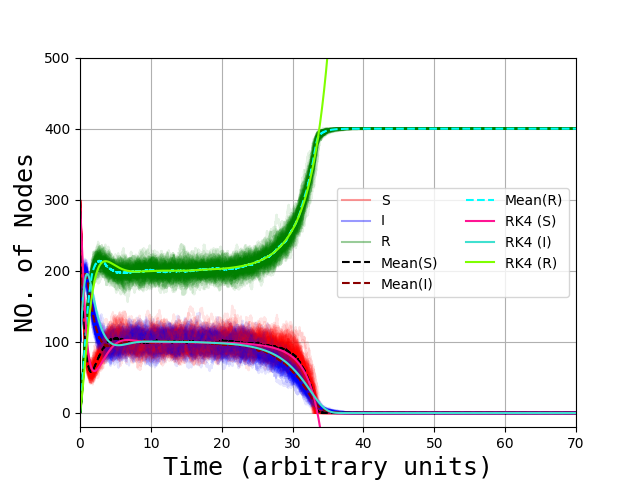
\includegraphics[width=1.1\linewidth]{Figures/Vax_expt_15x03_ckonst_4_1_05.png}
			\caption{Exponential vaccination, constant $\gamma$}
		\end{subfigure}
		\begin{subfigure}{0.49\linewidth}
		    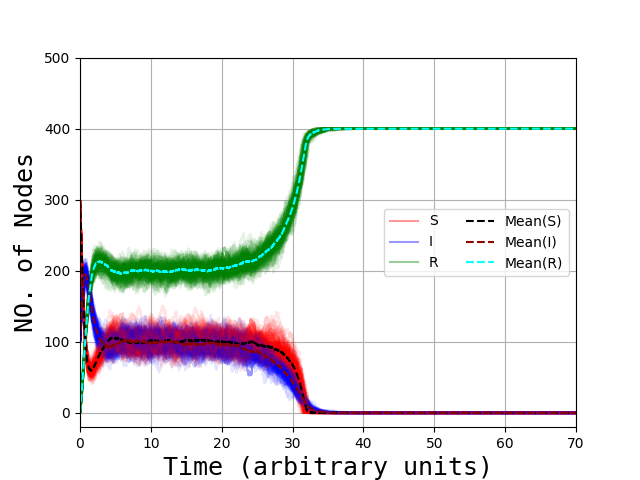
\includegraphics[width=1.1\linewidth]{Figures/Vax_expt_15x03_cvar_4_1_05.png}
			\caption{Exponential vaccination, variable $\gamma$}
		\end{subfigure}
		\caption{Development with vaccination with $\alpha = 4$, $\beta = 1$, $\gamma=0.5$ after time 10 for a and b and after time 15 for c and d}
		\label{fig:vaccinationvar}
	\end{figure}

Figure \ref{fig:vaccinationvar} displays the results obtained for simulations in which different vaccination programs are initiated after a given time $t$. In Figure \ref{fig:vaccinationvar} (b) we have implemented a function which decreases the rate of recovery $\gamma$ as discussed in Section \ref{section:vacfunc}, and the same was done in Figure \ref{section:vacfunc}. In these plots the ODE solutions are not included as the variable rate of recovery was never implemented for this solver. 

